\section{Auswertung}
\label{sec:Auswertung}

% \begin{figure}
%   \centering
%   \includegraphics{plots/plot.pdf}
%   \caption{Plot.}
%   \label{fig:plot}
% \end{figure}



% \begin{table}
%    % Notation :  {% nicht entfernen ist sehr wichtig sonst Fehler !!
% \parbox{0.48\textwidth}{% %Ermöglicht zwei Tabellen neben einander
%   \centering
%   \sisetup{round-mode = places , round-precision = 0,scientific-notation=fixed, fixed-exponent = 0}
%          %rundet Werte aus Stelle, Stelle = ,  macht einen bestimmten festen exponenten
%   \resizebox{\textwidth}{!}{%  % skaliert zu große Tabellen
%   \begin{tabular}{S@{${}\pm{}$} S} % fügt plus minus Fehler Schreibweise hinzu
%     \toprule
%      $\text{e}_b / \si{\milli\meter}$ &
%      $\text{d}_b /\si{\milli\meter} $ & $\text{f}_b / \si{\milli\meter} $\\
%     \midrule
%     \bottomrule
%   \end{tabular}
%   % }
%   \caption{Tabellenunterschrift}
%   \label{tab:tab}
% }
% % \end{table}
% % \begin{table}
% \parbox{0.48\textwidth}{%
%   \centering
%   \sisetup{round-mode = places , round-precision = 0,scientific-notation=fixed, fixed-exponent = 0}
%   % \resizebox{\textwidth}{!}{%
%   \begin{tabular}{S@{${}\pm{}$} S}
%     \toprule
%      $\text{e}_b / \si{\milli\meter}$ &
%      $\text{d}_b /\si{\milli\meter} $ & $\text{f}_b / \si{\milli\meter} $\\
%     \midrule
%     \bottomrule
%   \end{tabular}
%   % }
%   \caption{Tabellenunterschrift}
%   \label{tab:tab}
% }
% \end{table}
\paragraph{Bestimmung der maximalen Kraftflussdichte des mag. Feldes}
Zur Bestimmung der maximalen Kraftflussdichte, wird zu erst die Kraftflussdichte in ein 
Diagramm gegen die z-Position aufgetragen und dann mit einer Ausgleichskurve approximiert. 
Die Ausgleichskurve wurde mit nicht-linearer Ausgleichsrechnung unter Zurhilfenahme von 
\cite{scipy} und folgender Gaußfunktion bestimmt: 
\begin{equation}
	f(z)= \frac{A}{\sqrt{2\pi\sigma}}\cdot\exp\left(-\frac{1}{2} \left(\frac{z}{\sigma} \right) ^2 \right)
\end{equation} 
Daraus ergibt sich, dass $A= \SI{0.0096(4)}{\tesla\meter}$ und $\sigma = \SI{0.0084(4)}{\meter}$ 
betragen muss. An der Position der Probe ist die Kraftflussdichte maximal, also bei 
$z =0$, folglich ergibt sich, dass  die maximale Kraftflussdichte $f(0) = \SI{0.45(2)}{\tesla}$ 
beträgt. Das zuvor erwähnte Diagramm ist in der Abbildung \ref{fig:BFeld} zusehen, alle Werte 
dazu sind in der Tabelle \ref{tab:BFeld} dargestellt.
 \begin{figure}
   \centering
   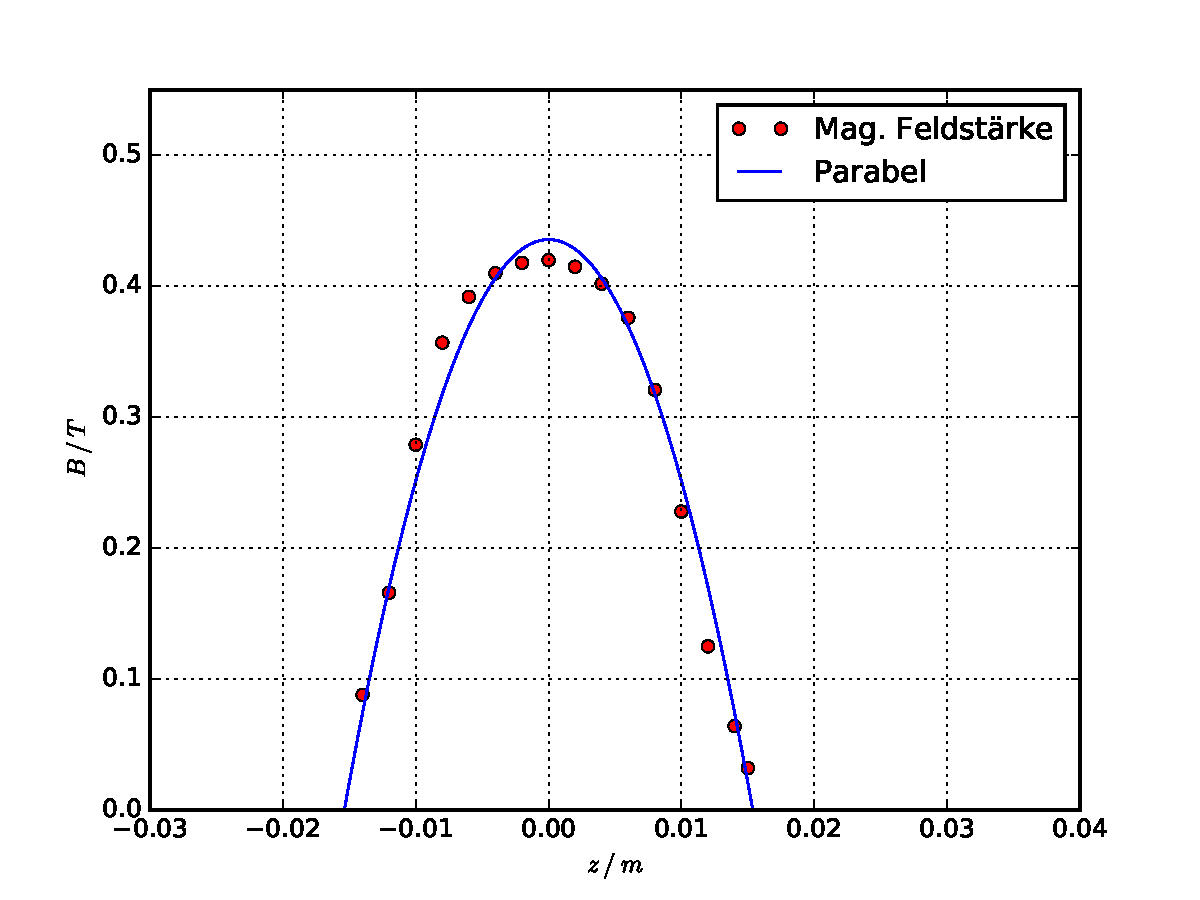
\includegraphics[height= 7cm]{plots/BFeld.pdf}
   \caption{Magnetische Feldstärke parallel zum Strahlengang. Die Probe liegt im Zentrum, hier bei Null. Der Verlauf der mag. Feldstärke wurde mit einer Gaußfunktion approximiert.}
   \label{fig:BFeld}
 \end{figure}

  \begin{table}
   \centering
   \sisetup{round-mode = places , round-precision = 3,scientific-notation=fixed, fixed-exponent = 0}
   \begin{tabular}{S S}
     \toprule
      $\text{Feldstärke} B /\si{\tesla} $ & $z \text{-Position} / \si{\meter} $\\
     \midrule
       8.799999999999999489e-02 & -1.400000000000000029e-02\\
       1.660000000000000087e-01 & -1.200000000000000025e-02\\
       2.790000000000000258e-01 & -1.000000000000000021e-02\\
       3.569999999999999840e-01 & -8.000000000000000167e-03\\
       3.920000000000000151e-01 & -6.000000000000000125e-03\\
       4.100000000000000311e-01 & -4.000000000000000083e-03\\
       4.179999999999999827e-01 & -2.000000000000000042e-03\\
       4.199999999999999845e-01 & 0.000000000000000000e+00\\
       4.150000000000000355e-01 & 2.000000000000000042e-03\\
       4.020000000000000240e-01 & 4.000000000000000083e-03\\
       3.760000000000000009e-01 & 6.000000000000000125e-03\\
       3.210000000000000075e-01 & 8.000000000000000167e-03\\
       2.280000000000000082e-01 & 1.000000000000000021e-02\\
       1.250000000000000000e-01 & 1.200000000000000025e-02\\
       6.400000000000000133e-02 & 1.400000000000000029e-02\\
       3.200000000000000067e-02 & 1.499999999999999944e-02\\
     \bottomrule
   \end{tabular}
   \caption{Werte zur Bestimmung der maximalen Kraftflussdichte.}
   \label{tab:BFeld}
  \end{table}

\paragraph{Faraday-Rotation an n-dotiertem und hochreinem GaAs}
Zuerst wurden die längennormierten Winkel der Faraday-Rotation gegen die quadrierte Wellenlänge 
aufgetragen, dies ist in der Abbildung \ref{fig:Vgl} zusehen. 

\begin{figure}
  \centering
  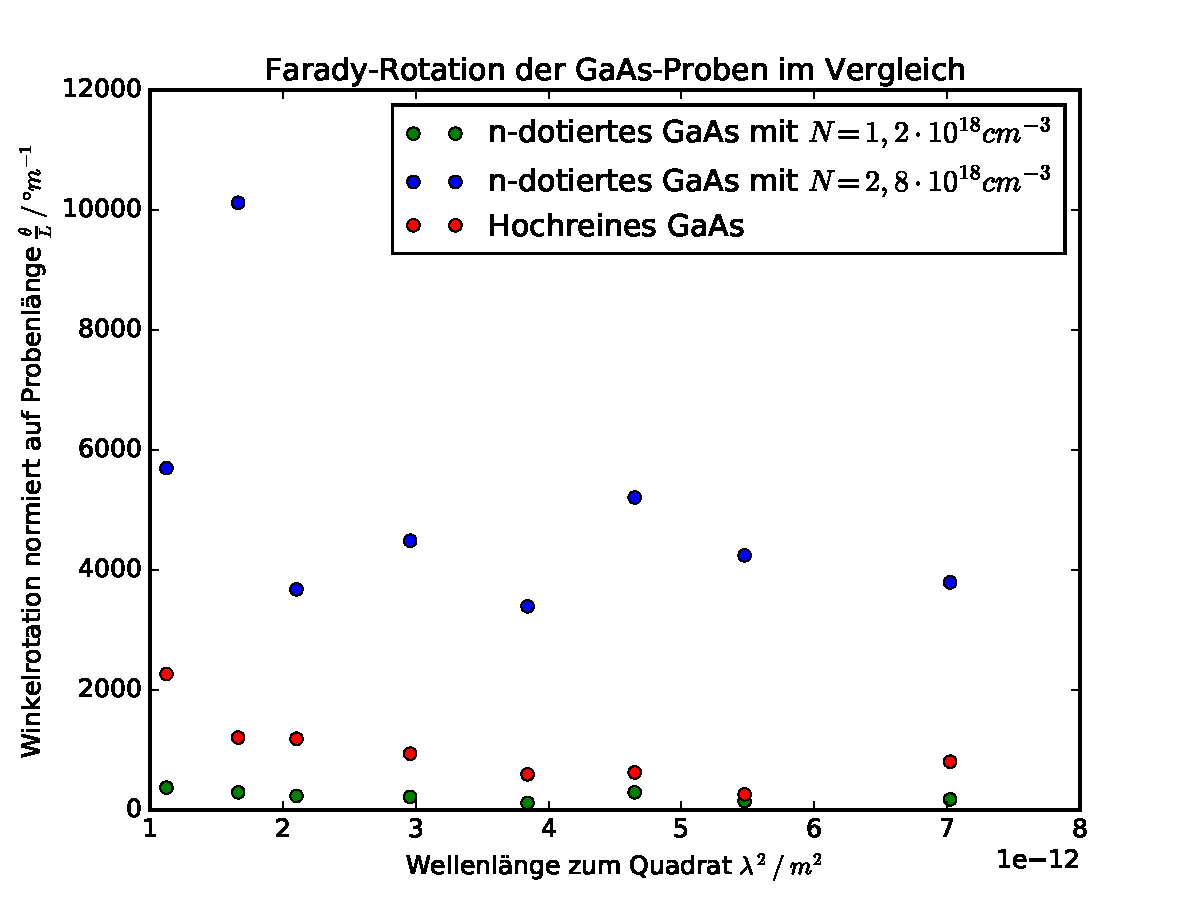
\includegraphics[height=7cm]{plots/GaAsimVgl.pdf}
  \caption{Die Längennormierte Farady-Rotation aller GaAs-Proben im Vergleich.}
  \label{fig:Vgl}
\end{figure}
